\documentclass[xetex,mathserif,serif]{beamer}
\usepackage{polyglossia}
\setdefaultlanguage[babelshorthands=true]{russian}
\usepackage{minted}
\usepackage{tabu}

\useoutertheme{infolines}

\usepackage{fontspec}
\setmainfont{FreeSans}
\newfontfamily{\russianfonttt}{FreeSans}

\tabulinesep=0.7mm

\title{Практика по рисованию поведенческих диаграмм}
\author[Юрий Литвинов]{Юрий Литвинов \newline \textcolor{gray}{\small\texttt{yurii.litvinov@gmail.com}}}

\date{05.04.2017г}

\begin{document}
	
	\frame{\titlepage}

	\begin{frame}
		\frametitle{Диаграммы случаев использования (или прецедентов)}
		\framesubtitle{Use case diagrams}
		\begin{center}
			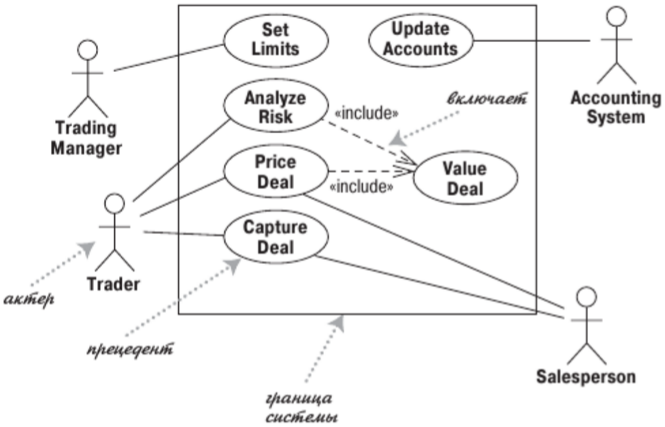
\includegraphics[width=0.6\textwidth]{useCaseDiagram.png}
		\end{center}
	\end{frame}

	\begin{frame}
		\frametitle{Задача 1}
		Нарисовать диаграмму случаев использования для своего проекта
	\end{frame}

	\begin{frame}
		\frametitle{Диаграммы активностей}
		\framesubtitle{Activity diagrams}
		\begin{center}
			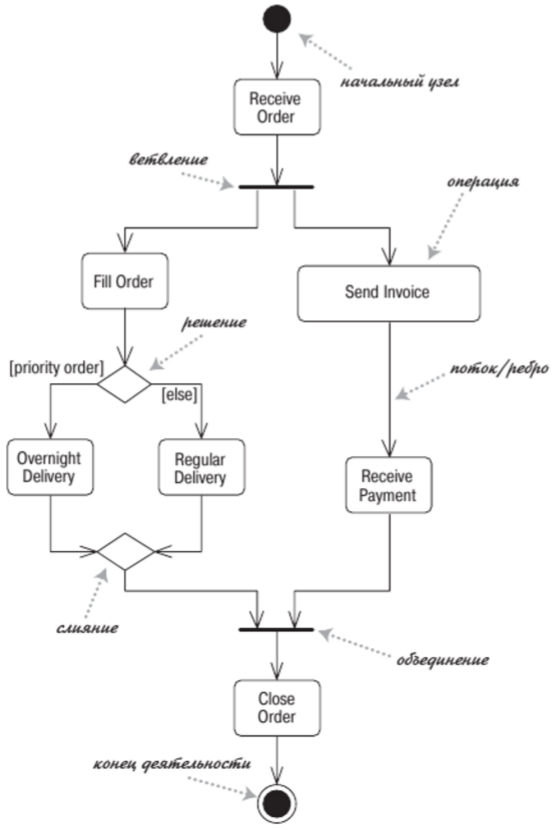
\includegraphics[width=0.415\textwidth]{activityDiagram.png}
		\end{center}
	\end{frame}

	\begin{frame}
		\frametitle{Диаграммы активностей, разделы}
		\framesubtitle{Swimlanes}
		\begin{center}
			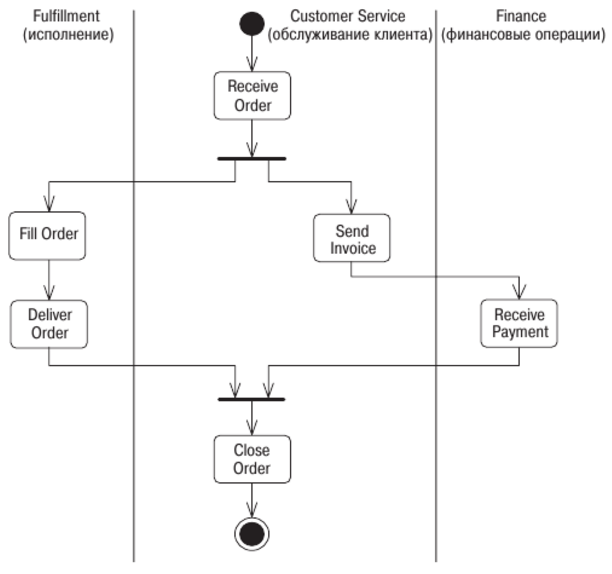
\includegraphics[width=0.55\textwidth]{activitySwimlanes.png}
		\end{center}
	\end{frame}

	\begin{frame}
		\frametitle{Диаграммы активностей, сигналы}
		\begin{center}
			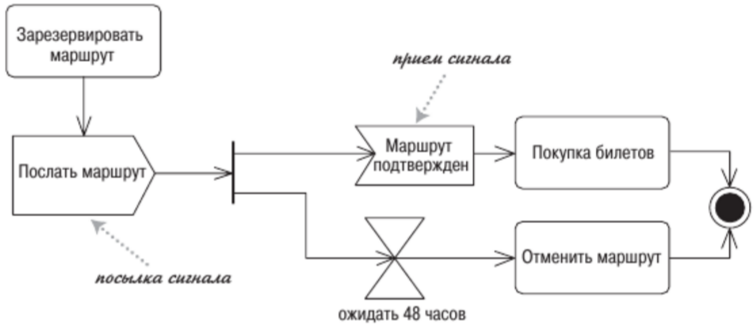
\includegraphics[width=0.7\textwidth]{activitySignals.png}
		\end{center}
	\end{frame}

	\begin{frame}
		\frametitle{Задача 2}
		Нарисовать диаграмму активностей для какого-либо сценария использования своего проекта
	\end{frame}

	\begin{frame}
		\frametitle{Диаграммы последовательностей}
		\framesubtitle{Sequence diagrams}
		\begin{center}
			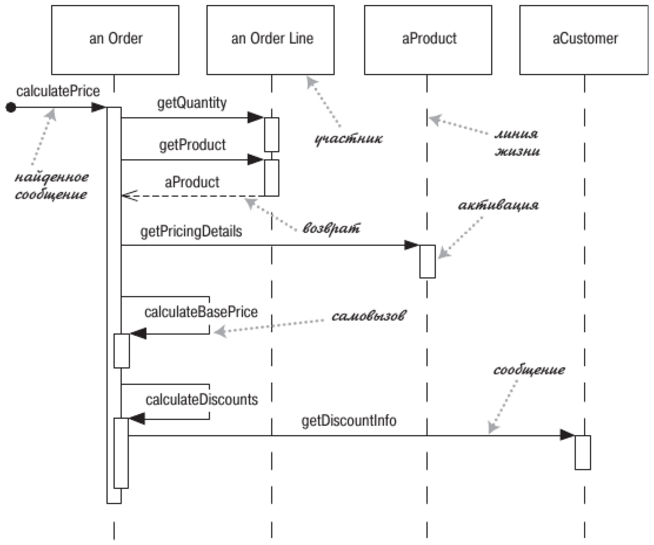
\includegraphics[width=0.6\textwidth]{sequenceDiagram.png}
		\end{center}
	\end{frame}

	\begin{frame}
		\frametitle{Диаграммы последовательностей, создание и удаление объектов}
		\begin{center}
			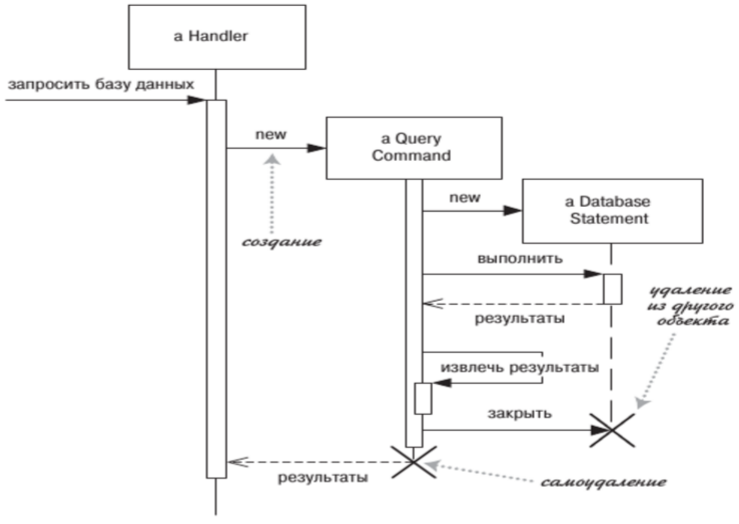
\includegraphics[width=0.65\textwidth]{sequenceLifeCycle.png}
		\end{center}
	\end{frame}

	\begin{frame}
		\frametitle{Диаграммы последовательностей, фреймы}
		\begin{center}
			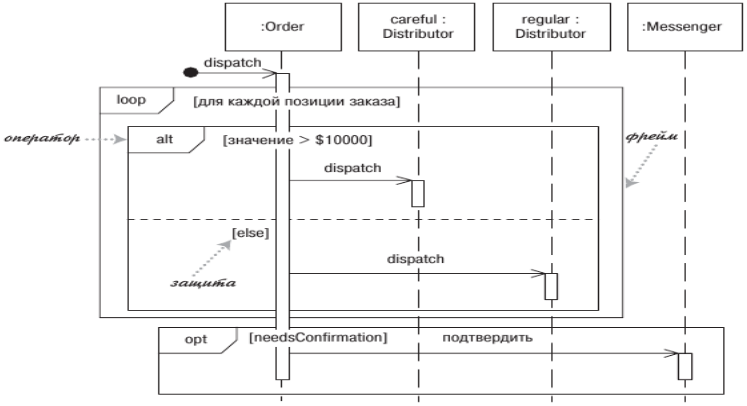
\includegraphics[width=0.8\textwidth]{sequenceFrames.png}
		\end{center}
	\end{frame}

	\begin{frame}
		\frametitle{Задача 3}
		Внезапно, нарисовать диаграмму последовательностей для какого-либо сценария для своего проекта
	\end{frame}

\end{document}
